\chapter{MInDes的配置,安装}\label{chap:install}

\section{运行环境}

本程序包可在 Windows 64位环境下以及 Linux 发行版 Ubuntu 上运行。运行时建议将系统更新至最新的版本。

\section{软件安装与初次运行}

以下将以 Windows 10 操作系统为例演示程序包的安装

可从\href{https://github.com/Microstructure-Intelligent-Design/Applications}{Github仓库}中下载程序包
Application-main.zip:

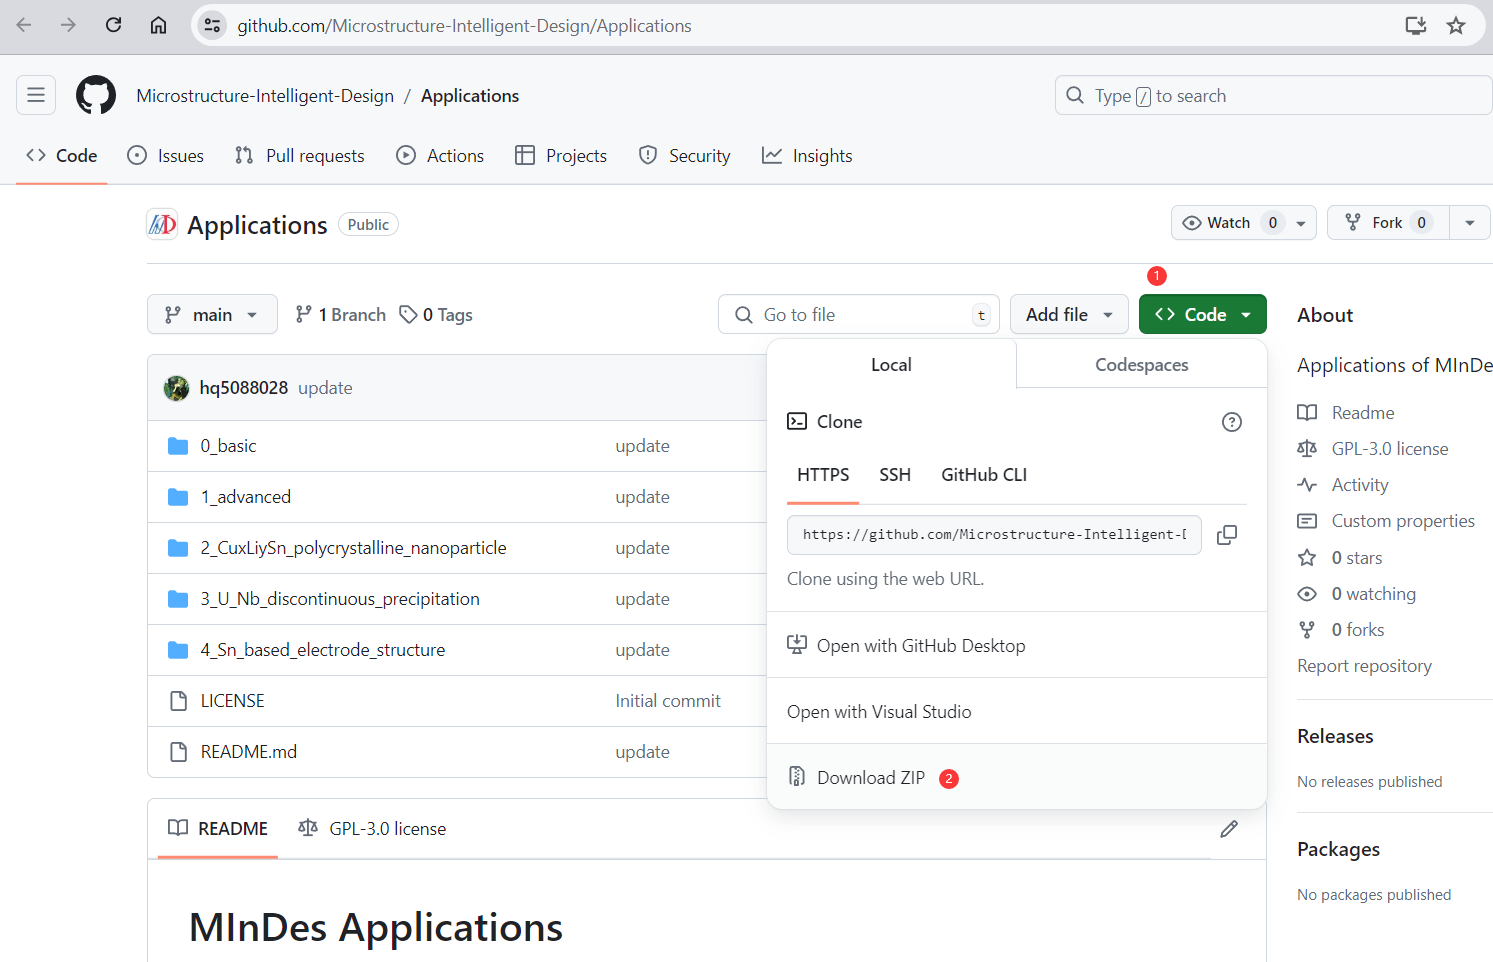
\includegraphics[width=5in]{rsc/download_mides.png}

随后将程序包解压缩,可得到以下文件:

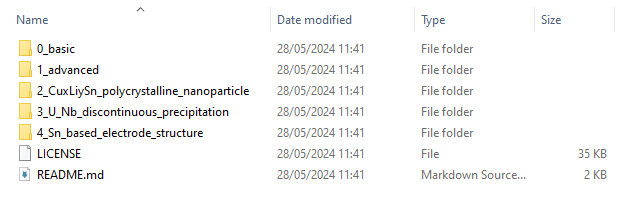
\includegraphics[width=5in]{rsc/mid_package_contents.png}

其中基本的输入文件位于文件夹 \emph{0\_basic} 中,其余应用案例位于后续文件夹中。
此处以 \emph{2\_CuxLiySn\_polycrystalline\_nanoparticle} 为例。

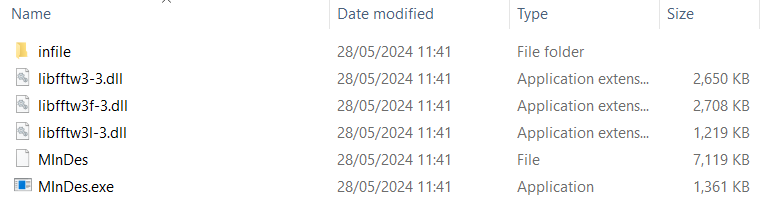
\includegraphics[width=5in]{rsc/example_folder.png}

自上而下分别为:\emph{infile}:输入文件所在文件夹;\emph{libfftw*.dll}:软件运行依赖;
\emph{MInDes}:Linix 系统执行程序;\emph{MInDes.exe}:Windows 系统执行程序。

于对应系统中运行可执行程序,即可进入软件配置界面:
\begin{itemize}
  \item {\color{magenta}Windows 环境下}:

        运行软件后键入\ \verb|i|\ 并回车,即可进入软件信息界面。\\
        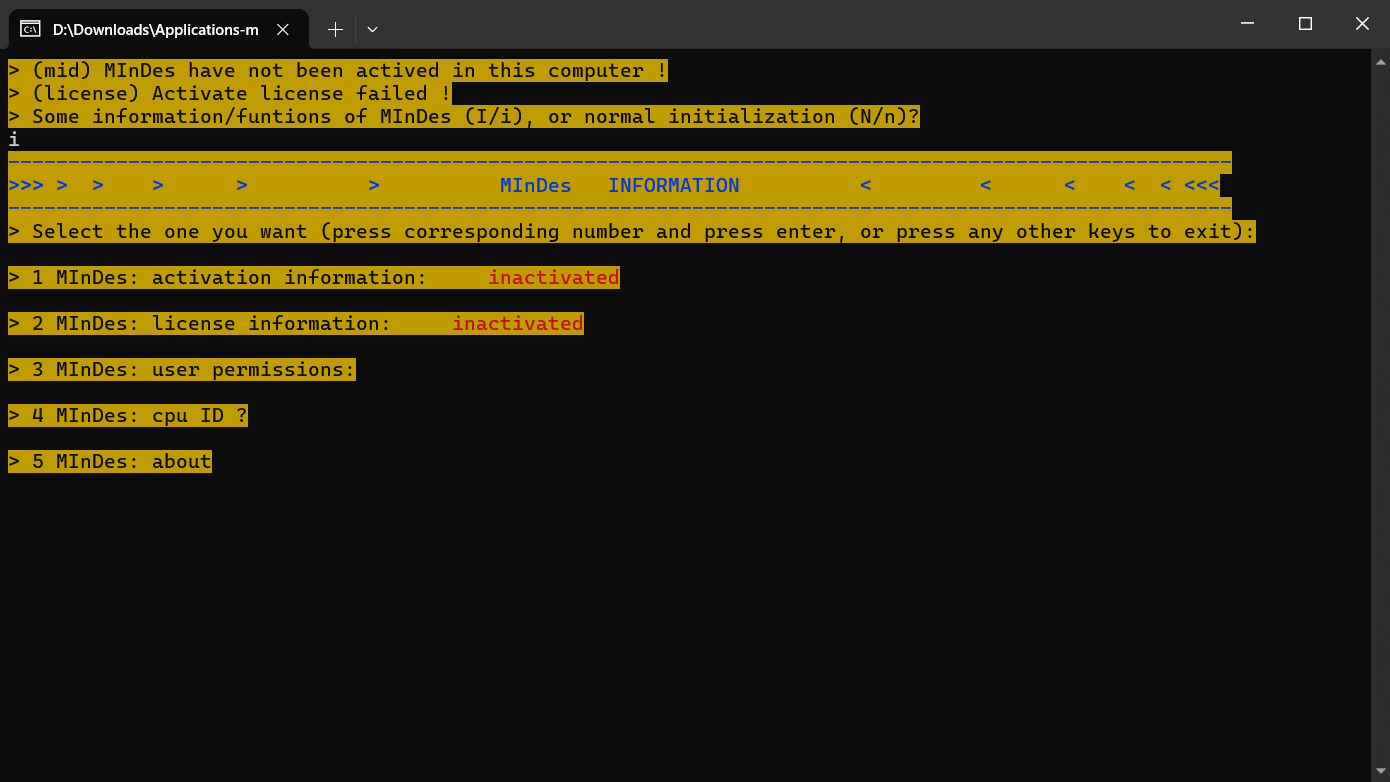
\includegraphics[width=5in]{rsc/mid_info_win.png}

  \item {\color{magenta}Linux 环境下}:

        无参数运行软件后将直接进入软件信息界面。\\
        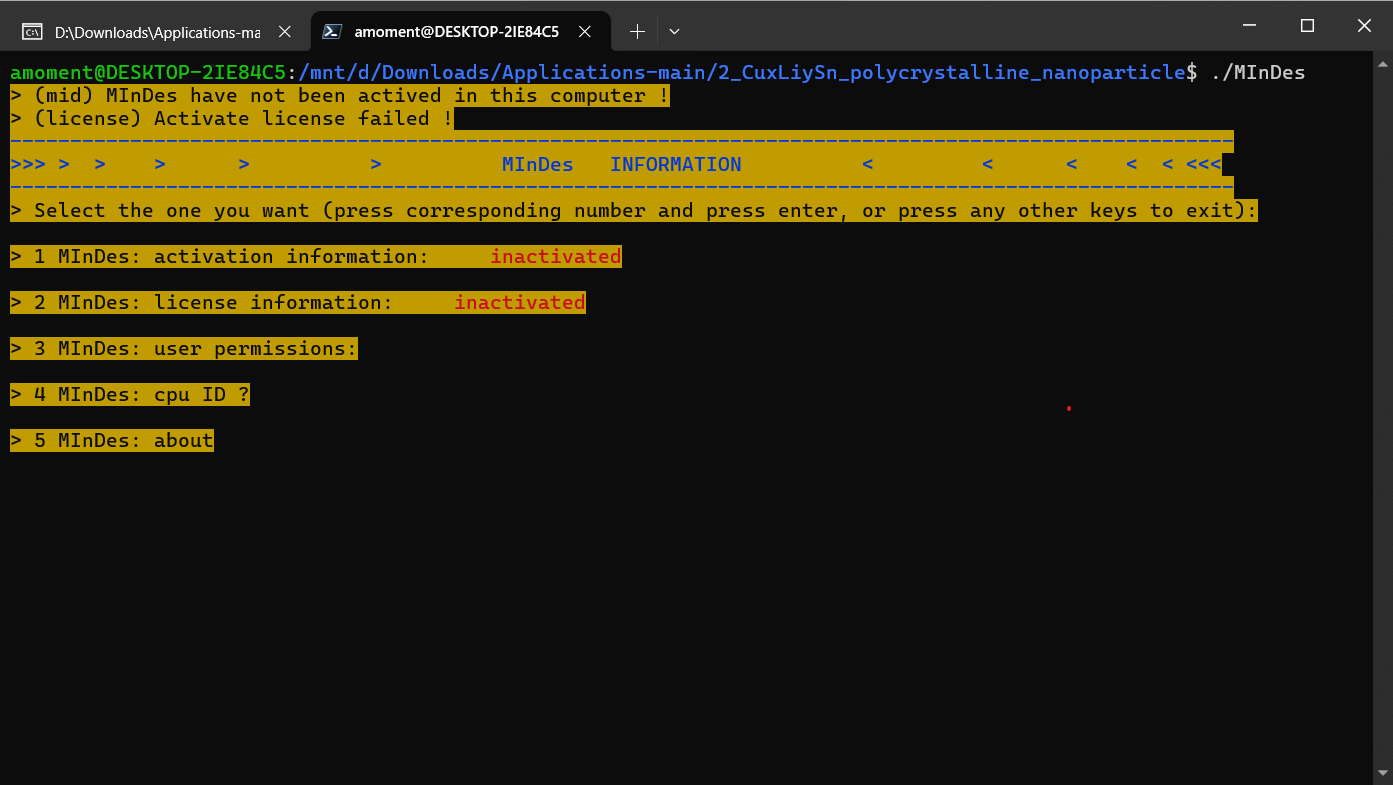
\includegraphics[width=5in]{rsc/mid_info_linux.png}

\end{itemize}
于此界面下,可以查看:(1)激活信息;(2)许可证信息;
(3)查看当前软件权限;(4)获取CPU ID;(5)查看软件概况(如下图)。

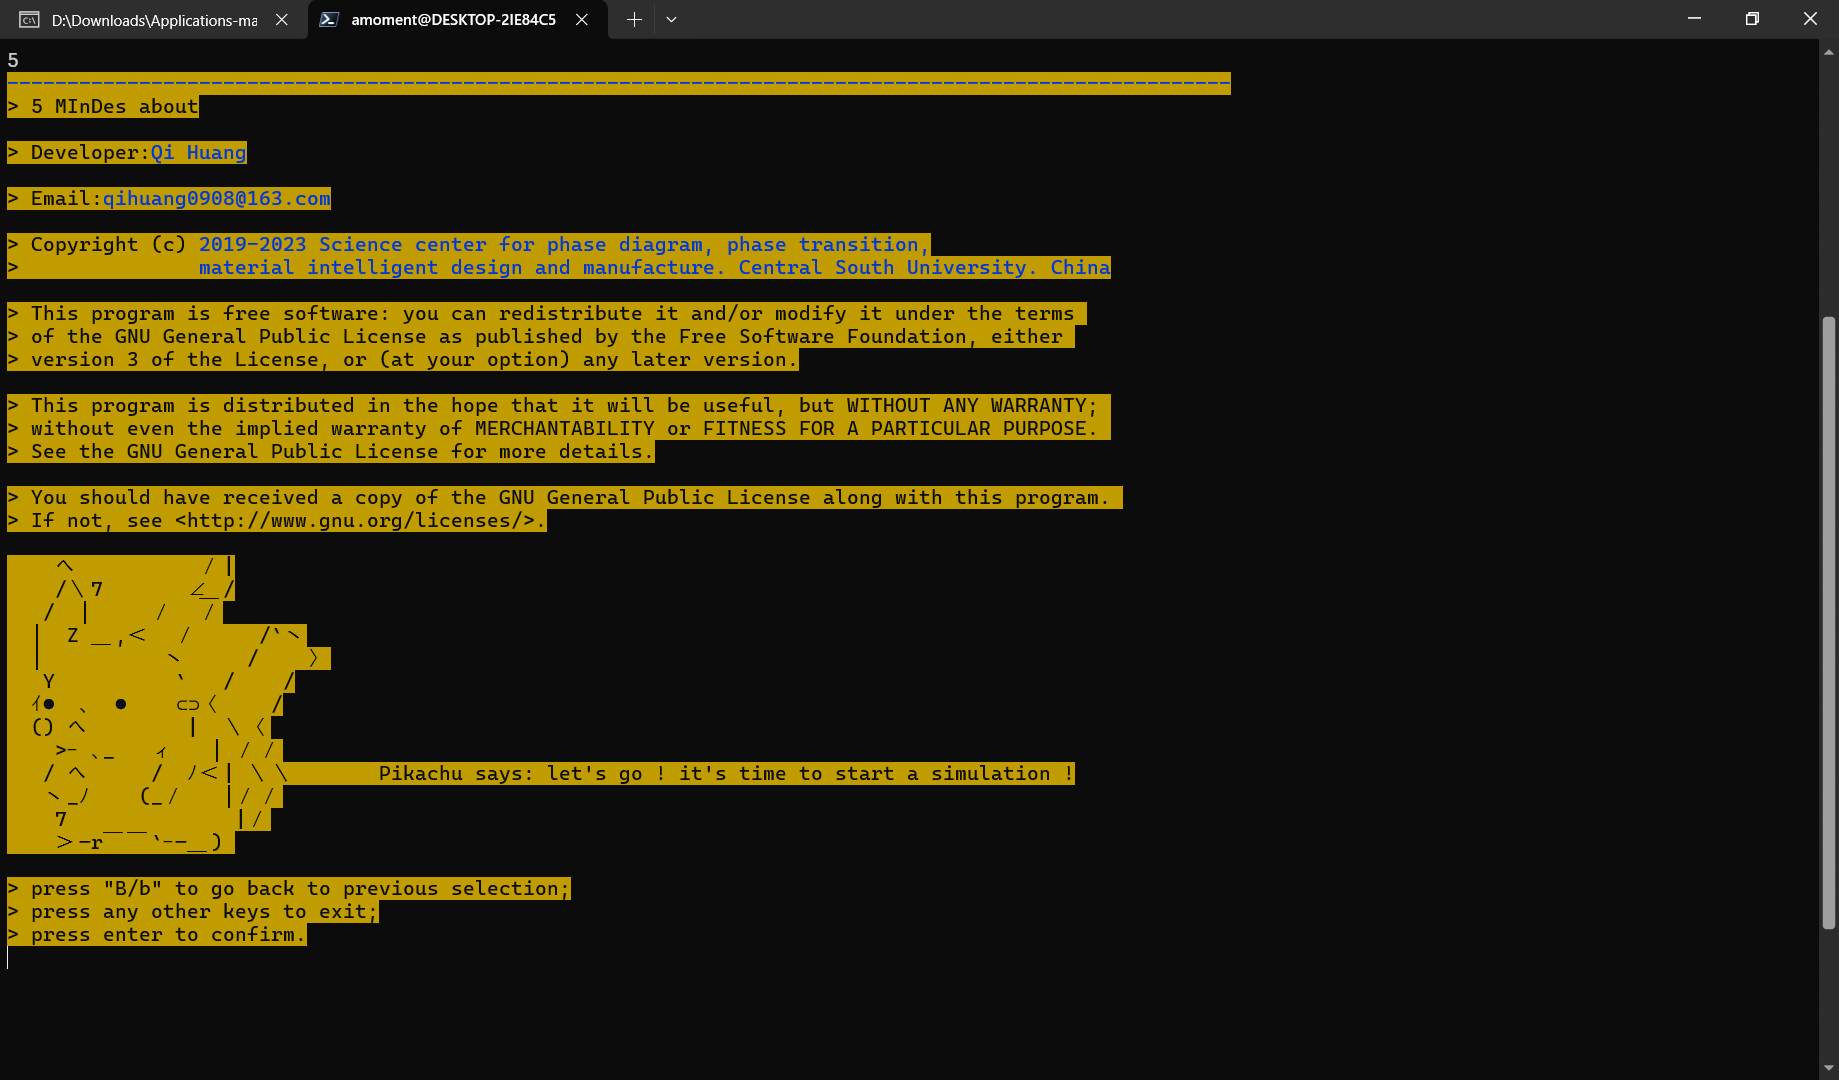
\includegraphics[width=5in]{rsc/mid_info_about.png}

\endinput
